  The main quantity of interest here is the jet fragmentation function. It characterizes the longitudinal fraction
  of the jet transverse momentum carried by charged particles:
    \begin{equation}
  z \equiv   \frac{\pttrk}{\ptjet} \cos \Delta R  
  = \frac{\pttrk}{\ptjet} \cos {\sqrt{\Delta \eta^2 + \Delta \phi^2}}
  \label{formula:z}
    \end{equation}
  $\Delta \eta$ and $\Delta \phi$ are the distance between the jet axis and the charged particle position in
  pseudorapidity and azimuth, respectively.
  $\Delta R$ is the distance between the particle and jet positions.
The fragmentation function is the distribution of the fragmentation variable, $z$, carried by the charged particle as illustrated in the Fig.~\ref{Fig:zdef} and it is defined as  

\begin{figure}
\centerline{
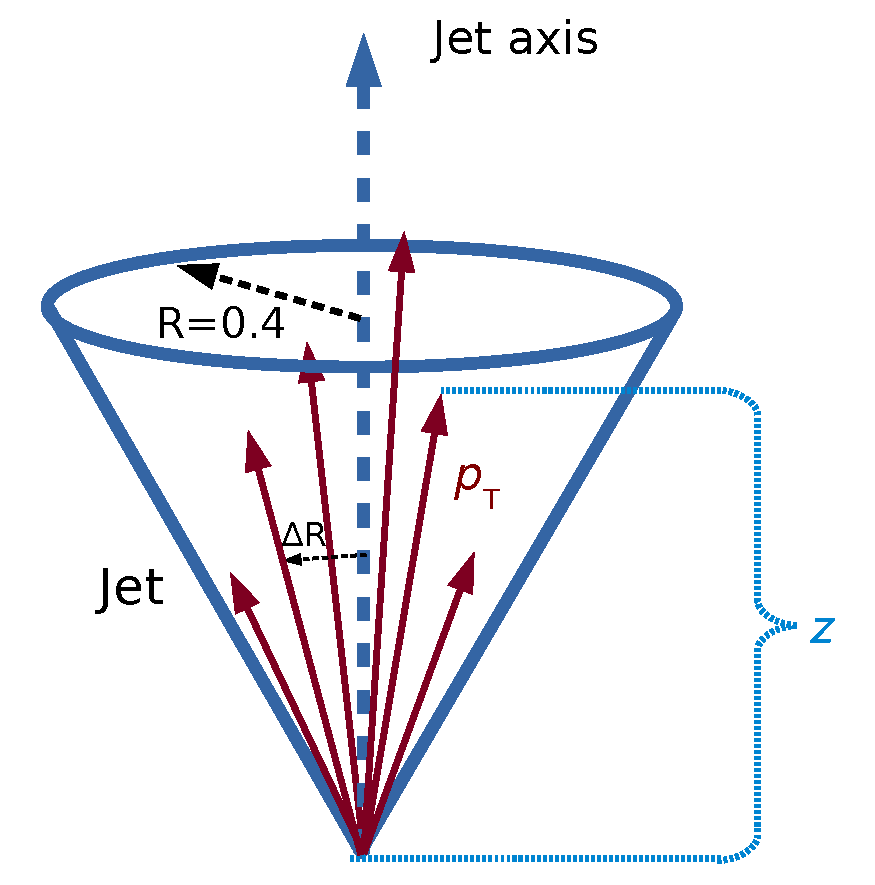
\includegraphics[width=0.55\textwidth]{figures_general/fragScheme_v2.pdf}
}
\caption{
Illustration of the jet fragmentation.    
  }
\label{Fig:zdef}
\end{figure}

\begin{equation}
D(z,\ptjet,y) = \frac{1}{N_{\mathrm{jet}}} ~ \frac{1}{\epsilon(\pttrk ,y)} ~ \frac{\mathrm{d} N_{\mathrm{ch}}}{\mathrm{d} z}~(\ptjet,y)
\end{equation}
where $N_{\mathrm{jet}}$ is number of jets in a given \ptjet\ bin, $N_{\mathrm{ch}}(z,\pTjet)$ is the number of charged particles with a maximum distance from the jet axis of $\Delta R \leq 0.4$ with given $z$, $y$ is jet rapidity, and $\epsilon(\pttrk ,\etatrk)$ is track $\pt$ and track $\eta$-dependent tracking efficiency. 
We also measure the \pt\ distribution of tracks within a jet.  This quantity, $D(\pt )$ is defined in
an analogous manner to $D(z )$:
\begin{equation}
D(\pt,\ptjet,y) = \frac{1}{N_{\mathrm{jet}}} ~ \frac{1}{\epsilon(\pttrk ,y)} ~ \frac{\mathrm{d} N_{\mathrm{ch}}}{\mathrm{d} \pt}~(\ptjet,y).
\end{equation}
This quantity is very close to the \Dz\ distributions only without the projection of the track \pt\ onto the jet axis and without the
scaling by \ptjet.
These distributions are potentially of interest if the interactions of the jet with the medium produced in \pbpb\ 
collisions introduce a characteristic \pt\ scale to the fragmentation function modification.  A similar measurement
has been made by CMS~\cite{Chatrchyan:2014ava}.



The measured fragmentation functions are affected by a contribution of tracks from the underlying event. The fragmentation function associated with the UE is evaluated separately. The subtracted $D(z)$ distribution is then evaluated as  
\begin{equation}
D(z,\ptjet,y) = \frac{1}{N_{\mathrm{jet}}(\ptjet,y)}  ~ 
\Bigg( 
\frac{1}{\epsilon(\pt ,\ptjet,y)} ~ \frac{\Delta N_{\mathrm{ch}}(z,\ptjet)}{\Delta z} - \frac{1}{\epsilon(\pt ,\eta_{\mathrm{trk}})} ~ \frac{\Delta N_{\mathrm{ch}}^{\mathrm{UE}}(z,\ptjet)}{\Delta z} 
\Bigg)
\end{equation}
and the subtracted $D(\pt)$ distribution is evaluated as
\begin{equation}
D(\pt,\ptjet,y) = \frac{1}{N_{\mathrm{jet}}(\ptjet,y)} ~ 
\Bigg( 
\frac{1}{\epsilon(\pt ,\ptjet,y)} ~ \frac{\Delta N_{\mathrm{ch}}(z,\ptjet)}{\Delta \pt} -  \frac{1}{\epsilon(\pt ,\eta_{\mathrm{trk}})} ~ \frac{\Delta N_{\mathrm{ch}}^{\mathrm{UE}}(\pt,\ptjet)}{\Delta \pt} 
\Bigg)
\end{equation}

Jets and tracks used in the evaluation of $D(z)$ distribution are subjected to various corrections and cuts that are described in the Sec.~\ref{sec:cuts_corrections}. The fragmentation functions evaluated using fully calibrated jets passing quality cuts and efficiency corrected tracks are used to calculate the ``raw'' distributions. The raw distributions are then unfolded to the particle level using two dimensional Bayesian unfolding method in \ptjet\ and \z\ or in \ptjet\ and \pttrk.

The analysis is performed differentially in jet \ptjet, jet rapidity $y$, and centrality.  The jet \ptjet\ bin size grows with increasing \ptjet\ to have a good statistics in the full range of the measurement and they are adopted from other ATLAS jet measurements~\cite{ATLAS276FFConf}. The following jet $y$ bins are used: $|y|<0.3$, $0.3<|y|<0.8$, $0.8<|y|<1.2$, and $1.2<|y|<2.1$. This binning is adopted from the~\cite{ATLAS276FFConf}. Two different binnings of the $D(z,\ptjet)$ and $D(\pt,\ptjet)$ are used. The $y$-inclusive measurement is performed with binning that has approximately two times more bins to increase the ability of detailed studies of the shapes of modifications in HI collisions.       

In order to quantify the differences between jet fragmentation in \pbpb\ collisions and \pp\ 
collisions, the ratios of the fragmentation functions in \pbpb\ collisions to those in \pp\ 
collisions are reported:
\begin{equation}
   R_{\Dpt} \equiv \frac{\Dpt_{\pbpb}}{\Dpt{\pp}}
\end{equation}
and
\begin{equation}
   R_{\Dz} \equiv \frac{\Dz_{\pbpb}}{\Dz{\pp}}.
\end{equation}
In the absence of modifications to jet fragmentation in \pbpb\ collisions both ratios will be unity.

